\documentclass[12pt]{article}
\usepackage{amsmath}
\usepackage{graphicx}
\title{Computational Statistics}
\date{}
\begin{document}

\section{Data}

We have 3 vector valued random variables. The ith index represents the values for site domain i for a particular lineitem. In the context on a MAB problem, each index represents a lever. The variables are defined as:
\begin{itemize}
	\item \textbf{n} - number of impressions served over given time period
	\item \textbf{c} - number of clicks on impressions over same time period 
	\item \textbf{a} - number of acquisitions over same time period
\end{itemize}

\section{Models}
We define 5 models to fit the data:

\subsection{Model 1 - 'pooled'} 
All levers are assumed to have the same payoff function. A useful baseline model. We assume a uniform Beta prior so that the MAP estimate of r is equivlanet to the MLE and is also an unbiased estimator. We gain as much information about lever 1 by looking at lever 2 as by looking at lever 1.

  \begin{align}
	a_i \sim Bin(r,n_i) \\
	\pi(r) = Beta(1,1)
  \end{align}

\subsection{Model 2 - 'independent estimation'} 
We assume that each lever has a completely independent payoff function. There is no information to be gained about lever 1 by looking at lever 2.

  \begin{align}
	a_i \sim Bin(r_i,n_i) \\
	\pi(r_i) = Beta(1,1)
  \end{align}

\subsection{Model 3} 
Here we assume a hierarchical model where the conversion rate for each lever is sampled from a Beta distribution with common $\alpha$, $\beta$ parameters across all levers. In a sense, this model lies somewhere between model 1 and model 2, in that data about lever 1 gives us some information about lever 2 via inference of $\alpha$, $\beta$ parameters. 

  \begin{align}
	a_i \sim Bin(r_i,n_i) \\
	r_i \sim Beta(\alpha,\beta) \\
	\pi(\alpha) = Unif(0,10000) \\
	\pi(\beta) = Unif(0,10000)
  \end{align}

\subsection{Model 4} 
Since acquisitions are rare events, we try to gain more information about a lever be modelling the click-through-rate separately from the conversions. Similarly to model 3, CTR and CVR have a hierarchical model.

  \begin{align}
	a_i \sim Bin(q_i,c_i) \\
	c_i \sim Bin(p_i,n_i) \\
	q_i \sim Beta(\alpha_q,\beta_q) \\
	p_i \sim Beta(\alpha_p,\beta_p) \\
	\pi(\alpha_q) = Unif(0,10000) \\
	\pi(\beta_q) = Unif(0,10000) \\
	\pi(\alpha_p) = Unif(0,10000) \\
	\pi(\beta_p) = Unif(0,10000) 
  \end{align}

When p and q are independent of each other, $a_i$ has distribution $Bin(p_iq_i,n)$ and $p_iq_i$ has distribution $Beta(a_i,n_i - a_i)$ (see 'Do Clicks Matter' for proof). This makes it equivalent to model 3 with different priors. The intuition here is that clicks are not informative - as much as they increase our belief in click through rate, they decrease our belief in the acquisition rate.

\subsection{Model 5}
Model 4 assumed that CTR and CVR are independent. Experience suggests that levers tend to perform well on both CTR and CVR or poorly on both. In other words, there tend to be 'clusters' of good and bad levers. Model 5 attempts to capture this with a beta-binomial mixture model. We use priors to bias one cluster towards being the poor performer, this helps avoid 'index switching' complications with model fitting. 
 
 \begin{align}
	a_i \sim Bin(q_i,c_i) \\
	c_i \sim Bin(p_i,n_i) \\
	k \sim Bern(h) 
\end{align}
	\[ 
	q_i \sim 
  	\begin{cases}
		Beta(\alpha_{q0},\beta_{q0}) & \quad \text{if k is 0}\\
		Beta(\alpha_{q1},\beta_{q1}) & \quad \text{if k is 1}
	\end{cases}
	\]
	\[
	p_i \sim 
  	\begin{cases}
		Beta(\alpha_{p0},\beta_{p0}) & \quad \text{if k is 0}\\
		Beta(\alpha_{p1},\beta_{p1}) & \quad \text{if k is 1}\\
	\end{cases}
	\]

 \begin{align}
	\pi(h) = Unif(0,1) \\
	\pi(\alpha_{q0}) = Gamma(1,2) \\
	\pi(\beta_{q0}) = Gamma(1,2) \\
	\pi(\alpha_{p0}) = Gamma(1,2) \\
	\pi(\beta_{p0}) = Gamma(1,2) \\
	\pi(\alpha_{q1}) = Unif(0,10000) \\
	\pi(\beta_{q1}) = Unif(0,10000) \\
	\pi(\alpha_{p1}) = Unif(0,10000) \\
	\pi(\beta_{p1}) = Unif(0,10000)
\end{align}

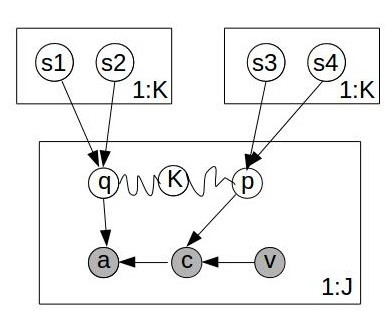
\includegraphics{GraphMod.jpg}

\section{Fitting Models}

For each model, we will generate a sample from the posterior distribution using the Stan modelling language.

If this becomes computationally infeasible, we may use point estimates or approximate inference techniques.

\section{Testing}

We will run the same tests on both an artificially generated dataset, as well as historical data from an Advance campaign.

The data from is randomly split between train and test datasets. Each model is fit using the training dataset and predictions compared against test data.

We define 3 loss functions:
\begin{enumerate}
	\item Posterior likelihood of realized CVR. See section 25.9 in the stan manual for how to use the generated quantities section to calculate posterior event probabilities.
	\item Volume weighted difference in realized CVR (relates closely to budget wasted). 
	\item Vol weighted MSE.
\end{enumerate}

\section{Do Clicks Matter}

\subsection{Distribution of a conditioned on n}

Firstly note that:

\begin{align}
{w+a \choose w}{n \choose w+a} &= \frac{n!}{(n-w-a)!w!a} \\
	&= \frac{n!(n-a)!}{((n-a)-w)!w!a!(n-a)!} \\
	&=  {n \choose a}{n-a \choose w}
\end{align}

We may construct the probability mass function for a using the conditional distributions:

\begin{align}
p(a|p,q,n) &= \sum_C p(a|q,c)p(c|p,n) \\
 &= \sum_{c=a}^n {c \choose a} p^a(1-p)^{c-a} {n \choose c} q^c (1-q)^{n-c}
\end{align}

Try to pull out a binomial by reparameterizing with $ w = c-a$:

\begin{align}
&= \sum_{w=0}^{n-a} {w+a \choose a} p^a(1-p)^w {n \choose w+a} q^{w+a} (1-q)^{n-w+a} \\
&= {n \choose a} (pq)^a \sum_{c=a}^n {n-a \choose w} ((1-p)q)^w (1-q)^{(n-a)-w} \\
&= {n \choose a} (pq)^a ((1-p)q +  (1-q))^{n-a} \\
&= Binom(a;pq,n)
\end{align}

Ref: http://math.stackexchange.com/questions/626457/conditional-binomials

\subsection{Posterior of qp}

We have now established that a is distributed as $Bin(qp,v)$. The question remains whether the uncertainty around the parameterization qp is reduced by modelling q and p separately.

For given a,c,n counts, p and q are independent. We therefore describe their joint density as.

\begin{align}
 f_{P,Q}(p,q) = Beta(p;c,n-c) Beta(q;a,c-a)
\end{align}

Using the same approach as 'Rao, Linear Statistical Inference and its Applications, 3a.3, pg 168' to get the density of pq, apply the following transformation:
\begin{align}
 u(p,q) = qp, \quad v(p,q) = q  \\
 \implies p(u,v) = \frac{u}{v}, \quad q(u,v) = v
\end{align}

\begin{align}
 f_{U,V}(u,v) &= f_{P,Q}(p(u,v),q(u,v)) 
		\frac{\partial p \partial q}{\partial u \partial v} 
		\text{ ,in range }  (u<v<1,0<u<1) \\
 &= Beta(v;c,n-c) Beta(\frac{u}{v};a,c-a) v^{-1} \\
 &= c . v^{c-1} (1-v)^{n-c-1} (\frac{u}{v})^{a-1} (\frac{v - u}{v})^{c-a-1} v^{-1} \\
 &= c . (1-v)^{n-c-1} u^{a-1} (v - u)^{c-a-1}
\end{align}

Now integrate out v. Noting that the integral has the form of a Beta function, we shift and scale the integral with a change of variable.

\begin{align}
\text{Choose }  w &= \frac{v-u}{1-u} \\
f_U(u) &= c.u^{a-1} \int_u^1 (1-v)^{n-c-1} (v - u)^{c-a-1} \mathrm{d}v \\
 &= c.u^{a-1} \int_0^1 ((1-w)(1-u))^{n-c-1} (w(1-u))^{c-a-1} (1-u) \mathrm{d}w \\
 &= c.u^{a-1} (1-u)^{n-a-1} B(n-c,c-a) \\
 &= Beta(u;a,n-a) = Beta(qp;a,n-a) 
\end{align}

\end{document}
